\chapter{Literature Review}



\section{Current State of the Art in grasping} % Not a good title!
Looking at recent demos for grasping functionality , including industrial applications. Everything presented should be at application and implementation stage.

\section{Existing platforms}

\subsection{Grippers}
There are a huge number of robotic gripper available both commercially and open source versions. These gripper vary widely from simplistic to very complex and from general purpose to having a very specific niche applications for which they were designed. It would be very difficult to complete a comprehensive review of all available grippers but this section introduces a subset, representative of the range of grippers developed to date. Grippers are generalised into categories based on their morphologies and real world examples of each are given.

\begin{itemize}
    \item Pincer Grippers \ref{fig:YouBot}, \ref{label:Robotiq85}, \ref{label:Hand-E}
    
    Pincer Grippers are one of the simplest types of gripper, but despite their simplicity they are capable of a wide range of tasks. This low complexity and large range of applications is why they are one of the most used gripper designs. Pincer gripper use 2 opposing fingers to apply a clamping force onto the object. They require low control complexity but can encounter problems if the object is too heavy or irregularly shaped.
    
    \item Higher DOF Finger grippers \ref{lbel:Robotiq3Finger}
    \item Humanoid Grippers \ref{fig:Sandia}, \ref{fig:James}, \ref{fig:Allegro}, \ref{fig:DLR Hand II}
    \item Suction Cup Grippers
    \item Other \ref{fig:Coffee Bean Gripper}
\end{itemize}

\begin{figure}
    \centering
    \begin{subfigure}{.3\linewidth}
        \centering
        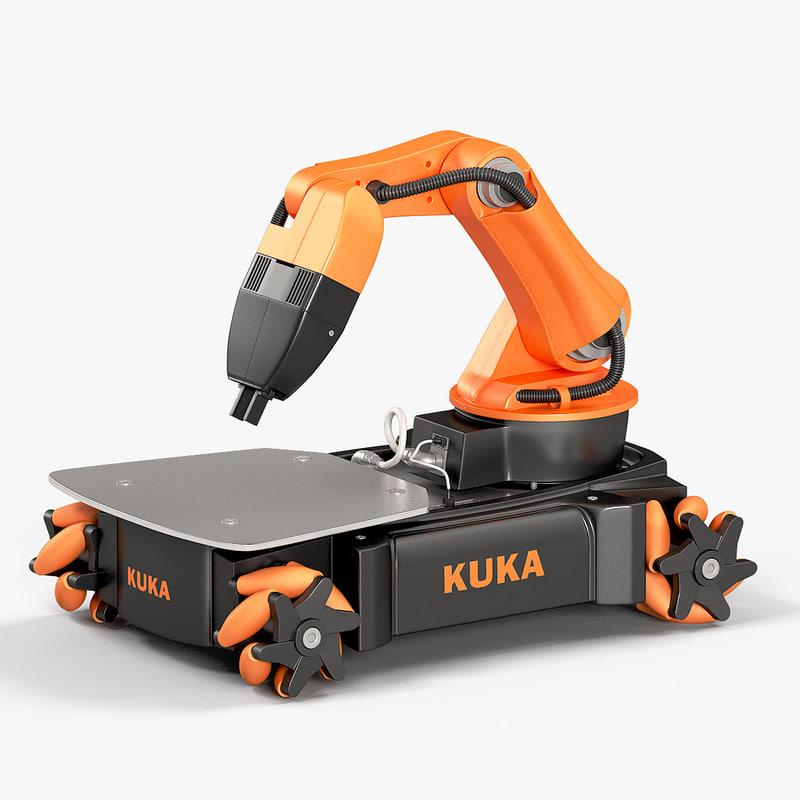
\includegraphics[width=0.7\textwidth]{Images/kuka-youbot-3D-model_0.jpg}
        \caption{YouBot}
        \label{fig:YouBot}
    \end{subfigure}
    \begin{subfigure}{.3\linewidth}
        \centering
        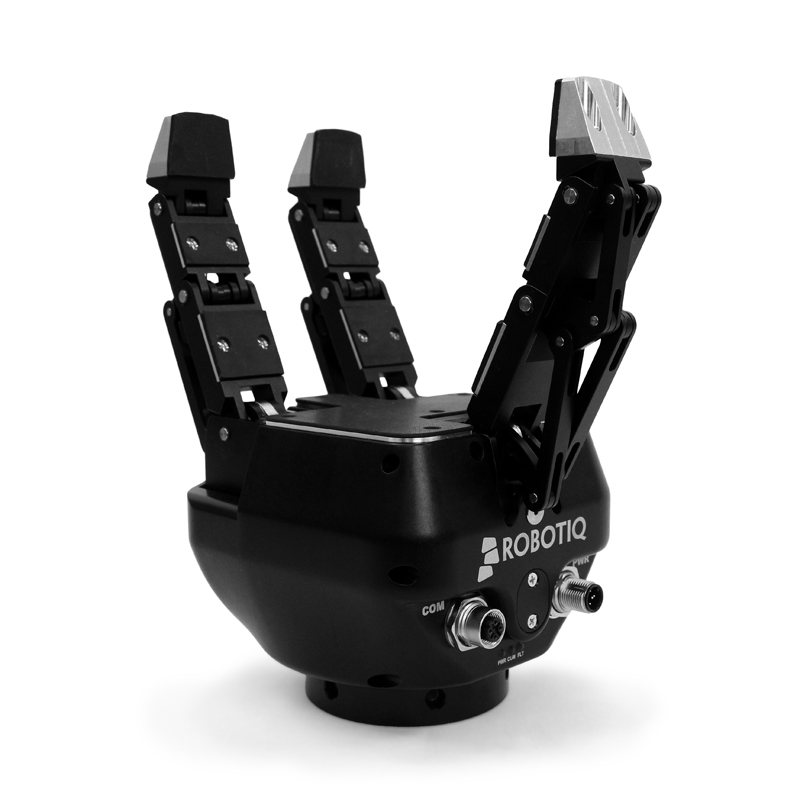
\includegraphics[width=0.7\textwidth]{Images/3-finger-robot-gripper-robotiq.jpg}
        \caption{3-Finger Adaptive Robot Gripper}
        \label{lbel:Robotiq3Finger}
    \end{subfigure}
    \begin{subfigure}{.3\linewidth}
        \centering
        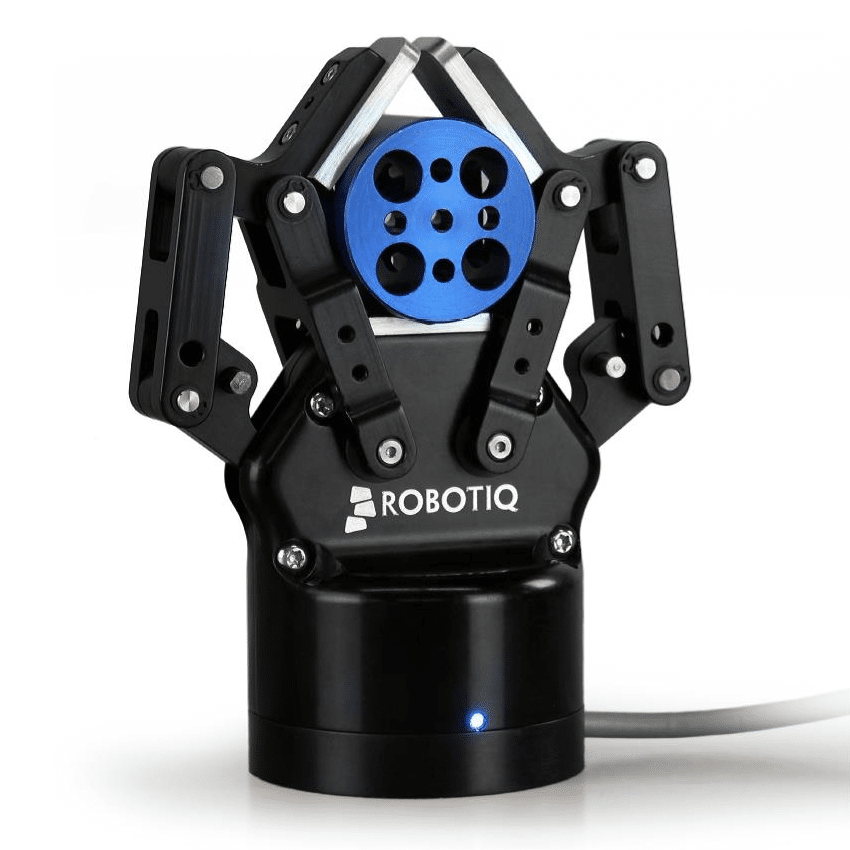
\includegraphics[width=0.7\textwidth]{Images/Robotiq-2-Finger-85-encompassing-grip.png}
        \caption{2F-85}
        \label{label:Robotiq85}
    \end{subfigure}
    \begin{subfigure}{.3\linewidth}
        \centering
        \includegraphics[width=0.7\textwidth]{Images/Hand£.png}           \caption{Hand-E}
        \label{label:Hand-E}
    \end{subfigure}
    \begin{subfigure}{.3\linewidth}
        \centering
        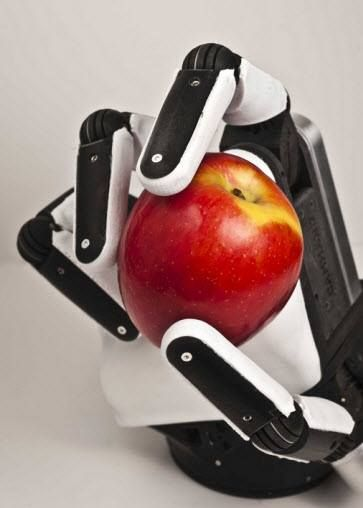
\includegraphics[width=0.7\textwidth]{Images/Sandia.jpg}        \caption{Sandia}
        \label{fig:Sandia}
    \end{subfigure}
    \begin{subfigure}{.3\linewidth}
        \centering
        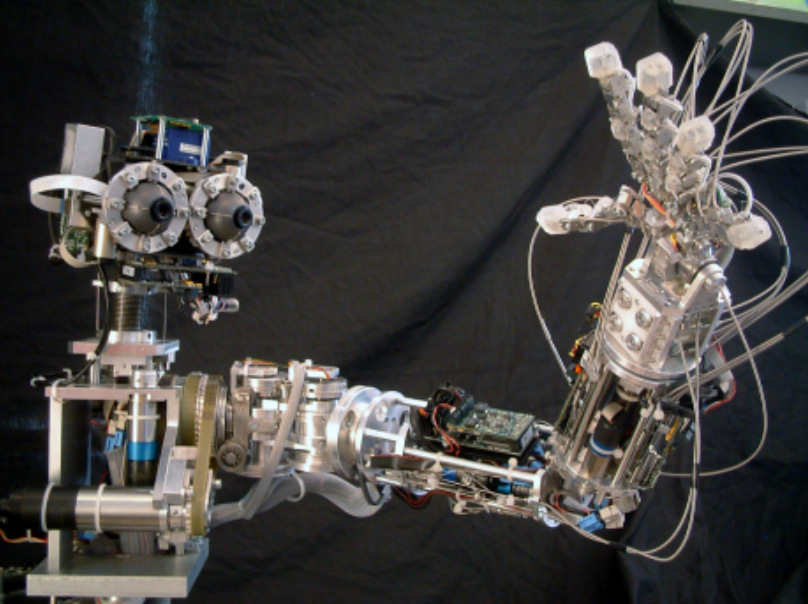
\includegraphics[width=0.7\textwidth]{Images/James.png}    \caption{James}
        \label{fig:James}
    \end{subfigure}
    \begin{subfigure}{.3\linewidth}
        \centering
        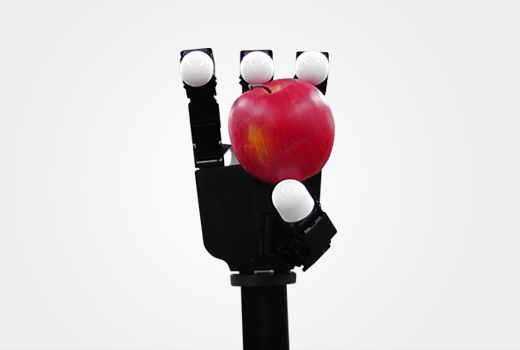
\includegraphics[width=0.7\textwidth]{Images/Allegro_Hand_flash_03.png}
        \caption{Allegro}
        \label{fig:Allegro}
    \end{subfigure}
    \begin{subfigure}{.3\linewidth}
        \centering
        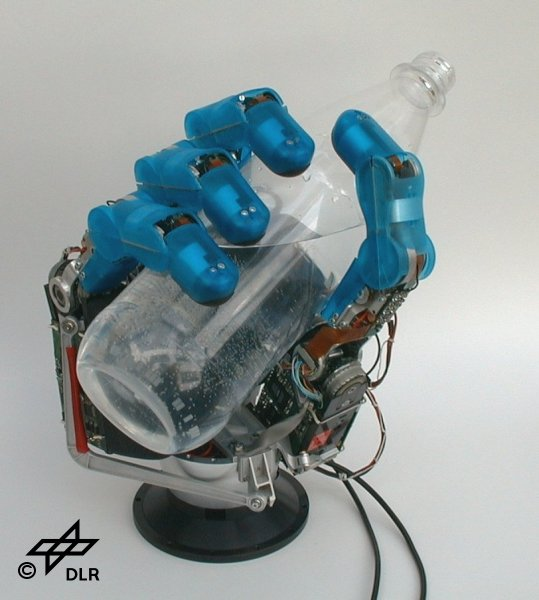
\includegraphics[width=0.7\textwidth]{Images/Hand-II-01.jpg}    \caption{DLR Hand II}
        \label{fig:DLR Hand II}
    \end{subfigure}
    \begin{subfigure}{.3\linewidth}
        \centering
        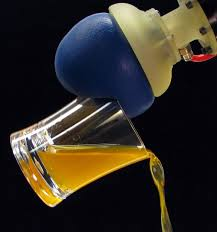
\includegraphics[width=0.7\textwidth]{Images/CoffeeBeanGripper.jpeg}    \caption{Coffee Bean Gripper}
        \label{fig:Coffee Bean Gripper}
    \end{subfigure}
\end{figure}

\subsection{Manipulators}
KUKA

\section{Grasp Sensing}

\subsection{Image}
Visual Camera
    RobotIQ, wrist camera
    
    
    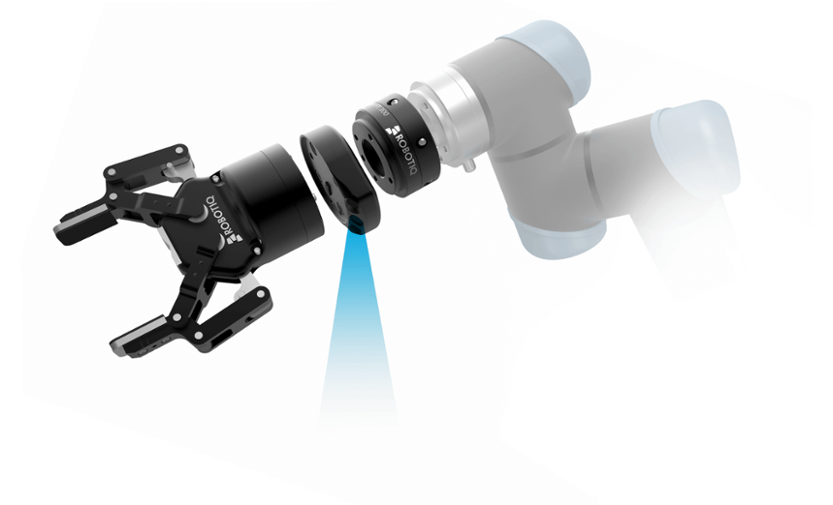
\includegraphics[width=0.2\textwidth]{Images/robotiq-vision-guided-robotic-hand-system.png}
Depth Camera
    APC 2016 Winners Delft

IR Sensing

\subsection{Tactile}
Hall Effect
Capacitive

\subsection{Joint Feedback}
Magnetic Encoders
Optical Encoders
Mechanical Encoders

\section{Actuation}
Actuation is a fundamental part of any manipulation system, the actuator is the component which enable the system to move. Broadly speaking the actuator will take some energy input, usually in the form of electrical or potential energy and convert that into kinetic energy. The actuator is essential for both moving the end effector into position and for the end effector to grasp the object. This section will look at the most common actuators used in robotic grippers to date, the advantages and disadvantages the trade off and the applications. This section will also look at actuation strategies, different ways to translate force or movement and examine the advantages and disadvantages of underactuated systems compared to fully actuated systems.

The first method of actuation examined is the DC motor. It is a very simple system where an electric potential input will cause a shaft to rotate. They are effective in a large range of sizes, inexpensive and efficient making them the most commonly used method of actuating any part of a robot. Despite this there are several disadvantages, DC motor produce maximum power and are most efficient at high speeds, this results in the use of gearboxs and other motion transmission methods which step down the speed while stepping up the torque. Although this trade off, more torque for less speed, is very advantageous for robotic applications there are inefficiencies and errors associated with these devices. Friction, noise and backlash are all problems which are introduced while making the system more expensive. Backlash in particular is a problem for robotic manipulation %% << H. Kawasaki and T. Komatsu, “Development of an anthropomorphic robot hand driven by built-in servo-motors,” in Proc. 3rd Int. Conf. ICAM, vol. 1, 1998, pp. 215–220.>>
, in order to maximize the number of poses which the manipulator can position and orientate its end effector in a manipulator generally has a large number of Degrees of Freedom (DOF). Similarly to maximise the flexibility of a gripper it also has a large number of DOF. In both cases these DOF are arranged in a relatively long open kinematic chain. The effect that blacklash and any other error between the desired and actual joint angle is that these error propigate and are amplified through the chain such that small relative errors caused by backlash at each joint causes a large absolute error in the position of the end effector.

A further disadvantage of using simple DC motors is the absence of a feedback mechanism. Generally the speed of a DC motor is determined by the voltage applied (neglecting the back emf in its coil) and the output torque is proportional to the current. Due to variations in these parameters it is difficult to determine the position of the motor at any particular time. Furturemore using the inputs to a DC motor as a way of determining the position of a robot joint is subject to error propigation since the volage input determines speed and in robotic manipulation we are generally interested in joint position. For example a small error in the estimation of the motor speed would cause the accumulation of a large error in the motor and therefore joint position over time.

Stepper Motors are another common method of actuation in robotics. They are similar in some ways to a simple DC motor but overcome some of the challenges while introducing a few also. Like a simple DC motor a stepper motor takes DC electricity as an input and produces kinetic energy in the form of a rotating shaft. The internal differences between a simple DC motor and a stepper motor is outside the scope of this document but in effect the mechanism by which a stepper motor operates allows it to be positionally controlled unlike its speed controlled brother the simple DC motor. This ability to control the position of the motor comes at the cost of requiring some kind of logic to control the motor, generally a micro-controller.

Beyond being able to set the position of a stepper motor there are several other advantages. Steppers motors exhibit holding torque which other DC motors cannot achieve, this means that aswell as being able to move a shaft it can also hold a shaft in position, a feature which is often used in manipulation applications.

Piezo electrics
Pneumatics
Artificial Muscles
Hydraulics

\subsection{Under Actuation}
Underactuation is a technique often used in robotics, among the mostly commonly sited reasons to choosing to underactuate a system is to reduce the number of actuators required \cite{UnderactuationReductionInActuactors}, to simplify the control and therefore computational overhead and to fully take advantage of the system's natural dynamic characteristics. 

A system is said to be underactuated if the number of dimensions in which it is free to move, i.e. its Degrees of Freedom (DOF) is more than the number of independently actuated joints. Most robots can be described by 

\begin{equation}
\ddot{q} = f_1(q,\dot{q},t) + f_2(q, \dot{q},t)u   
\end{equation}

where \(u\) is the control vector, \(t\) is time and the robot's state can be described by a vector of positions (\(q\)) and velocities(\(\dot{q}\)). In this more mathmatical formulation if 

\begin{equation}
    rank[f_2(q,\dot{q},t)] < dim[q]
\end{equation}

then the system is said to be underactuated.

More specific to robotic grippers underactuation can often be a desirable quality and give the grasper a degree of self adaptability.  

using elastic or flexible of elastic material to mechanically couple joints in the figure can allow the gripper to better adapt to the shape of an object and increase the chances of a successful grasp simply by carefully designing and utilising the physical embodiment of the hand.

\section{Grasping Strategies}
Sense Plan Act - Delft APC winners 20160

\section{Computation}

\section{Grasping Moving Objects}
Grasping dynamic objects adds another significant challenge to the manipulation problem but there are some examples of research and success in this area. The research to date can be broken down into three different levels of difficulty mainly based on how much is known about the object and its trajectory.

\begin{enumerate}
    \item Regular Object, controlled trajectory
    \item Irregular object, controlled trajectory
    \iten Regular object, uncontrolled trajectory
    \item Irregular object, uncontrolled trajectory 
\end{enumerate}

\begin{figure}
    \centering
        \begin{subfigure}
            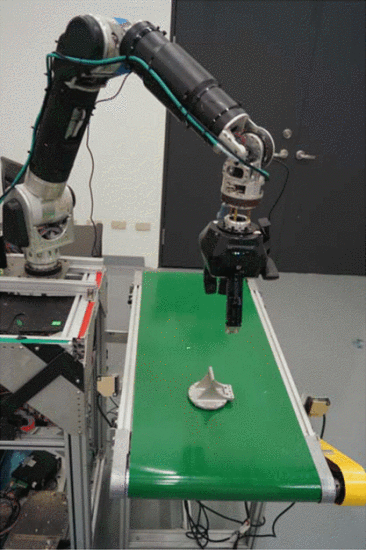
\includegraphics[]{Images/ConveyorBelt}
            \label{fig:Coffee Bean Gripper}
        \end{subfigure}
    \caption{Caption}
    \label{fig:my_label}
\end{figure}
